\documentclass[11pt, a4paper]{article}

%%% SST LAB PROTOCOLL PREAMBLE
%%% 2019
%%%%%%%%%%%%%%%%%%%%%%%%%%%%%%%


%%% PACKAGES
%%%%%%%%%%%%%%%%%%%%%%%%%%%

\usepackage[ngerman]{babel}

\usepackage[utf8]{inputenc}
\usepackage{amsmath}
\usepackage{pgfplots}
\usepackage{tikz}
\usepackage[many]{tcolorbox}
\usepackage{graphicx}
\graphicspath{ {./graphics/} }
\usepackage{pdfpages}
\usepackage{dashrule}
\usepackage{float}
\usepackage{siunitx}
\usepackage{trfsigns}
\usepackage{booktabs}
\usepackage[european]{circuitikz}
\usepackage{tcolorbox}

%%% DOCUMENT GEOMETRY
%%%%%%%%%%%%%%%%%%%%%%%%%%%

\usepackage{geometry}
\geometry{
 a4paper,
 total={0.6180339887498948\paperwidth,0.6180339887498948\paperheight},
 top = 0.1458980337503154\paperheight,
 bottom = 0.1458980337503154\paperheight
 }
\setlength{\jot}{0.013155617496424828\paperheight}
\linespread{1.1458980337503154}

\setlength{\parskip}{0.013155617496424828\paperheight} % paragraph spacing


%%% COLORS
%%%%%%%%%%%%%%%%%%%%%%%%%%%

\definecolor{red1}{HTML}{f38181}
\definecolor{yellow1}{HTML}{fce38a}
\definecolor{green1}{HTML}{95e1d3}
\definecolor{blue1}{HTML}{66bfbf}
\definecolor{hsblue}{HTML}{00b1db}
\definecolor{hsgrey}{HTML}{afafaf}

%%% CONSTANTS
%%%%%%%%%%%%%%%%%%%%%%%%%%%
\newlength{\smallvert}
\setlength{\smallvert}{0.0131556\paperheight}


%%% COMMANDS
%%%%%%%%%%%%%%%%%%%%%%%%%%%

% differential d
\newcommand*\dif{\mathop{}\!\mathrm{d}}

% horizontal line
\newcommand{\holine}[1]{
  	\begin{center}
	  	\noindent{\color{hsgrey}\hdashrule[0ex]{#1}{1pt}{3mm}}\\%[0.0131556\paperheight]
  	\end{center}
}

% mini section
\newcommand{\minisec}[1]{ \noindent\underline{\textit {#1} } \\}

% quick function plot
\newcommand{\plotfun}[3]{
  \vspace{0.021286\paperheight}
  \begin{center}
    \begin{tikzpicture}
      \begin{axis}[
        axis x line=center,
        axis y line=center,
        ]
        \addplot[draw=red1][domain=#2:#3]{#1};
      \end{axis}
    \end{tikzpicture}
  \end{center}
}

% box for notes
\newcommand{\notebox}[1]{

\tcbset{colback=white,colframe=green1!100!black,title=Note!,width=0.618\paperwidth,arc=0pt}

 \begin{center}
  \begin{tcolorbox}[]
   #1 
  \end{tcolorbox}
 
 \end{center} 
 
}

% box for equation
\newcommand{\eqbox}[2]{
	
	\tcbset{colback=white,colframe=green1!100!black,title=,width=#2,arc=0pt}
	
	\begin{center}
		\begin{tcolorbox}[ams align*]
				#1
		\end{tcolorbox}
		
	\end{center} 
	
}
% END OF PREAMBLE

\newcommand{\dBm}{\si{\deci\bel}\text{m}}

\begin{document}

\section{Vorbereitungsaufgaben}
\subsection{Funktionsweise einer BER-Messung}
Ein Pattern(Muster-)generator generiert Signal-Zufallsfolgen mit einer bestimmten
Periodenlänge und Datenrate. Diese Zufallsbitfolgen werden auf den Eingang des DUT/SUT gegeben. Am Empfänger ist die Zufallsfolge ebenfalls bekannt (z.B. durch
eigene Berechnung), sodass die Fehlerbits gezählt und daraus die BER
berechnet werden kann. Zur Synchronisation von Sender- und Empfänger
ist dafür eine Taktleitung notwendig. Optimalerweise sind Sender- und
Empfängereinheit in einem gemeinsamen Gerät vorhanden. Dies ist jedoch z.B.
bei der Messung von bereits installierten Strecken nicht gegeben, weshalb
zusätzlich auf die Qualität (Zeitverzögerung) des Taktsignals geachtet
werden muss.

\subsection{Auswirkung einer Erhöhung der Streckendämpfung auf die BER}
Eine höhere Dämpfung der Strecke führt zu einer verringerung der
Empfangsleistung und somit des Abstandes zwischen den vom Empfänger zu
unterscheidenden Logikpegeln. Das Empfangsauge verkleinert sich in vertikaler
Richtung und die Bitfehlerrate erhöht sich.


\subsection{Auswirkung einer vergrößerten Dispersion auf die BER}
Die Dispersion wirkt sich allgemein über unterschiedliche
Guppenlaufzeiten im Lichtwellenleiter durch eine Impulsverbreiterung am Empänger
aus und verkleinert somit das Empfangsauge in horizontaler Richtung,
wodurch die BER erhöht (ISI) und eine niedrigere Übertragungsrate für
die gleiche BER erforderlich wird.

\subsection{Dominierende Dispersionsart bei SM-Strecken}
Die Dispersion kann unterschieden werden in Materialdispersion und
Modendispersion. Da sich die Lichtausbreitung im SM-LWL auf eine einzige Mode
beschränkt (Grundmode) tritt dort auch keine Modendispersion auf, wodurch
nur die Materialdispersion verbleibt.

\subsection{Richtungsabhängigkeit der BER-Messung}
Eine Richtungsabhängigkeit der Messung liegt vor. Da der Laser einen
bestimmten Modenfeldradius besitzt, wird bei schlechter Kopplung (Offset)
das Signal am Anfang des Systems stärker negativ beeinflusst.

\subsection{Maximale BER}
Die maximal mögliche BER ist $0.5$.
Unter der Annahme von gaussverteiltem Rauschen lässt sich die
BER aus dem Signal-zu-Rausch-Verhältnis (SNR) über
\[\text{BER} = \frac{1}{2} \cdot \text{erfc}(\frac{\sqrt{SNR}}{2\sqrt{2}})\]
berechnen. Im worst case Fall strebt das Signal-Rauschverhältnis gegen 0,
wodurch die BER zu $0.5$ wird.

\subsection{Systemreserve}
Bei der Planung einer LWL-Strecke müssen mögliche Fehlerquellen im späteren
Betrieb berücksichtigt werden, um auch im Fall der erhöhten Dämpfung die
vorgesehene BER nicht zu überschreiten. Dämpfungserhöhungen können auftreten
durch z. B.
\begin{itemize}
  \item Alterungsprozesse der Spleiße
  \item Bauelementalterung (Empfänger, HL-BE etc.)
  \item Senderalterung (Laser)
\end{itemize}

Um solche Dämpfungserhöhungen abzufangen, dimensioniert man die LWL-Strecke mit
einer zusätzlichen Systemreserve, d.h. die zulässige Dämpfung wird künstlich
verringert und die Anforderungen an die Strecke somit erhöht. Eine heute gängige
Systemreserve ist $2 \, \si{\deci\bel}$.

\subsection{Dispersion Power Penalty}
Der Einfluss der Dispersion in einem vom idealen System abweichenden (zero-
length) System führt dazu, dass die Sendeleistung erhöht werden muss, um
gegenüber dem zero-length System die gleiche BER zu erreichen. Diese
Leistungserhöhung / Verschiebung ist die Dispersion Power Penalty (DPP).

\section{Versuchsaufgaben}

\begin{figure}[H]
  \centering
  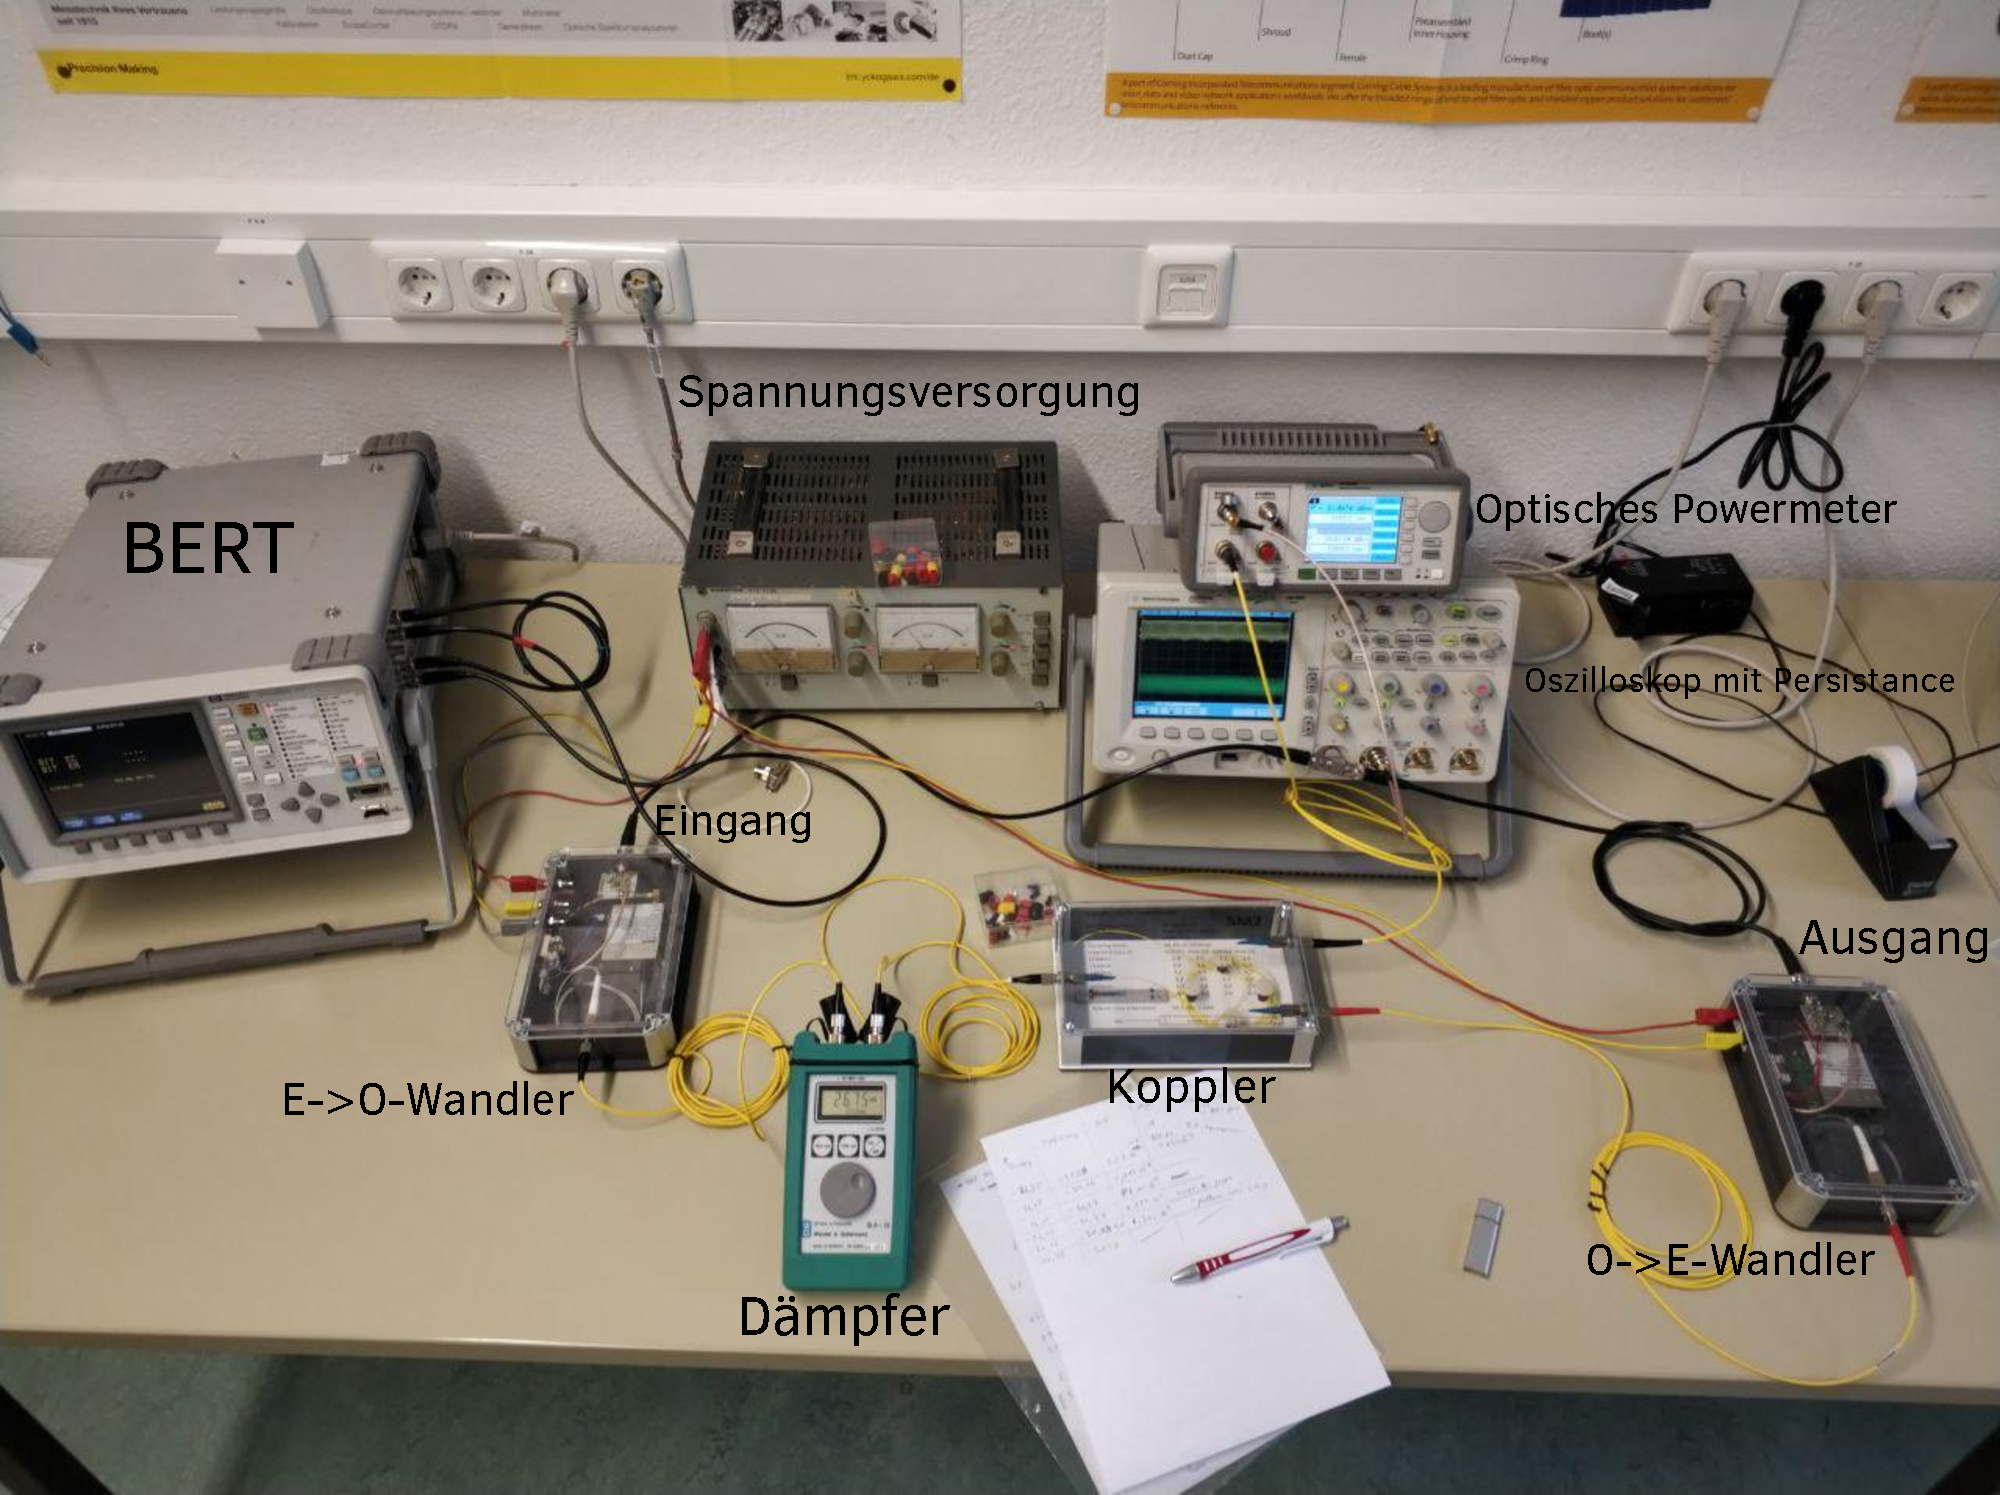
\includegraphics[width=\textwidth]{graphics/beepop}
  \caption{Versuchsaufbau zur BER-Messung}\label{aufbau}
\end{figure}

Der Versuch wurde bei einer Datenrate von $34 \, \si{\mega\bit\per\second}$ und
einer Wellenlänge von $1550 \, \si{\nano\meter}$ durchgeführt. Ein Optical
Attenuator (Dämpfer) sollte dabei die Leitungslänge simulieren, indem er eine
einstellbare Dämpfung in den Signalpfad einbringt. Der Nachteil dieser Methode
ist jedoch, dass der Einfluss der Dispersion auf die BER nicht untersucht werden
konnte. Der komplette Versuchsaufbau ist in Abb. \ref{aufbau} zu sehen.\\

Das BER-Testgerät sendet zufällige Bitfolgen im Frame von $15 \, \si{\bit}$ mit
TTL-Pegeln an einen elektrisch-optischen Wandler, welche dann über die
Strecke (und weiteren in Abb. \ref{aufbau} zu sehende Elementen) an das
Testgerät zurückgelangen und nach einer Messdauer von $30 \, \si{\second}$
ausgewertet werden. Zusammen mit der Bitrate ergibt das eine Gesamtbitzahl von
\[b = 34 \, \si{\mega\bit\per\second} \cdot 30 \, \si{\second} = 1.02 \,
  \si{\giga\bit}\]
Auf der Ausgabe erscheint dann die Fehlerzahl sowie die
berechnete BER.

\subsection{Bestimmung der Ausgangsleistung des Sendermoduls}\label{41}
Als Referenzpunkt für alle folgenden Messungen wurde eine Dämpfung von $3 \,
\si{\deci\bel}$ am Attenuator eingestellt. Die hinter dem $3 \si{\deci\bel}$-
Kopler gemessene Leistung ist
\[P_{\text{empf}}(a=3\si{\deci\bel}) = -8.239 \, \dBm\]

Dies entspricht der Leistung, die auch am Eingang des optisch-elektrischen
Wandlers anliegt und hier als grundlegende Sendeleistung angenommen wird.

\subsection{Bestimmung der minimalen Empfangsleistung des Empfängermoduls}
Die Dämpfung wurde so lange erhöht, bis die Bitfehlerrate am Empfänger den
Grenzwert von $10^{-9}$ erreicht hat, welcher einen gewöhnlichen Grenzwert für
Telekommunikationsanwendungen darstellt\footnote{https://www.fiberoptics4sale.com/blogs/archive-posts/95047174-what-is-ber-bit-error-ratio-and-bert-bit-error-ratio-tester}.
Die folglich gemessene Empfangsleistung beträgt
\[P_{\text{empf}} = -27.08 \, \dBm\]
In Bezug auf die Referenz-Sendeleistung aus \ref{41} ergibt sich ein Abfall von
\[\Delta = -8.239 \,\dBm - (-27.08 \,\dBm) = 18.841 \, \si{\deci\bel}\]

Dieser kann als zulässige Dämpfung der Strecke zur Einhaltung der BER von
$10^{-9}$ gedeutet werden.


\subsection{Bestimmung der BER in Abhängigkeit der optischen Empfangsleistung}
Beginnend bei einer BER von $10^{-9}$ wurde die Dämpfung in Schritten von $0.1
\, \si{\deci\bel}$ erhöht und die korrespondierende Empfangsleistung aufgenommen.


\end{document}
